
\begin{frame}
    \frametitle{Natural Language Processing and Mathematical Language}
    \begin{itemize}
        \item Natural language processing has benefitted from a long tradition of annotation tasks and benchmarks
        \item STEM documents pose problems:
            formulae, tables, \textellipsis
            \com{not really unicode strings}
        \item Why care?\\
            $\leadsto$ Semantic services
    \end{itemize}
\end{frame}


\begin{frame}
    \frametitle{Motivation: semantic services}
    \faSearch\;\; $\bm{1.5\,\text{\bf eV}}$
    \\[1em]
        \quad\quad\faExternalLink\;\; $1.43 \pm 0.9\,\text{eV}$\\[1em]
        \quad\quad\faExternalLink\;\; $2.4 \cdot 10^{-19}\,J$

    \vspace{3em}
    \faSearch\;\; $\bm{\sum_{k=-\infty}^\infty \text{\bf exp}(-\pi k^2)}$
    \\[1em]
        \quad\quad\faExternalLink\;\; $\sum_{n=-\infty}^\infty e^{-\pi n^2} = \ldots$
\end{frame}


\begin{frame}
    \frametitle{Motivation: semantic services}
    \hfill \examplecite{krisciunas2022including}\par
    \centering
    \begin{tikzpicture}
    \node at (0, 0) {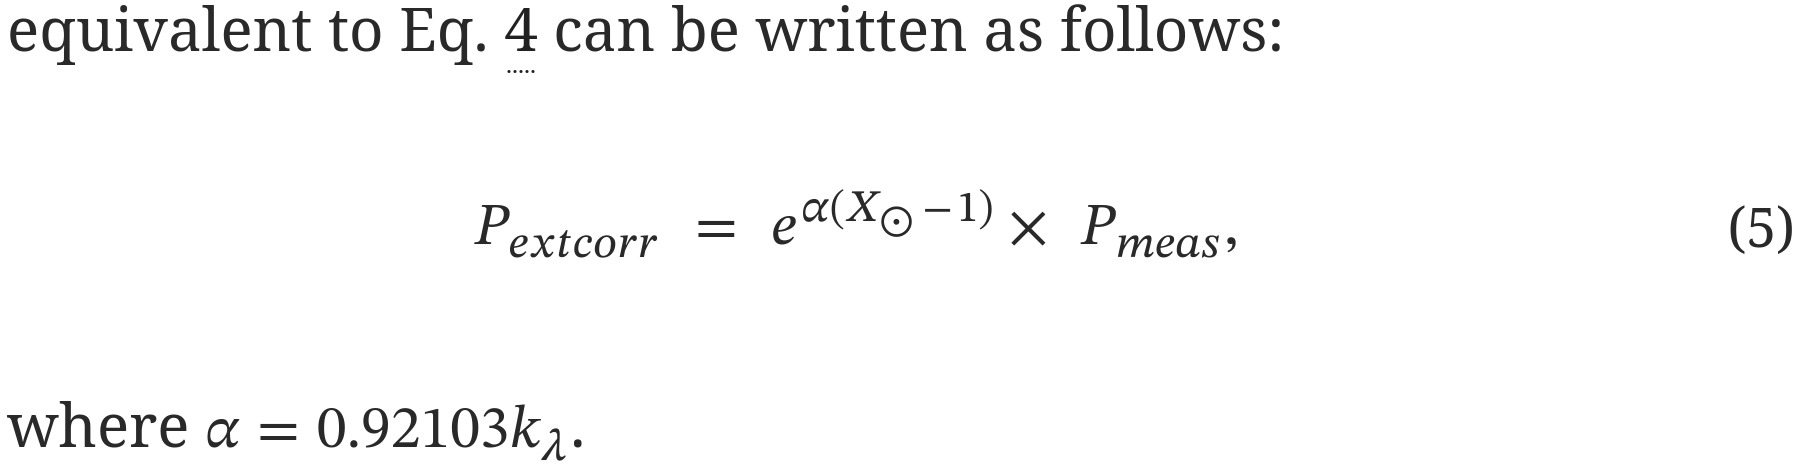
\includegraphics[width=0.8\textwidth]{extcorr_2107.02876.png}};
    \onslide<2>{\node at (1.6, -1.6) {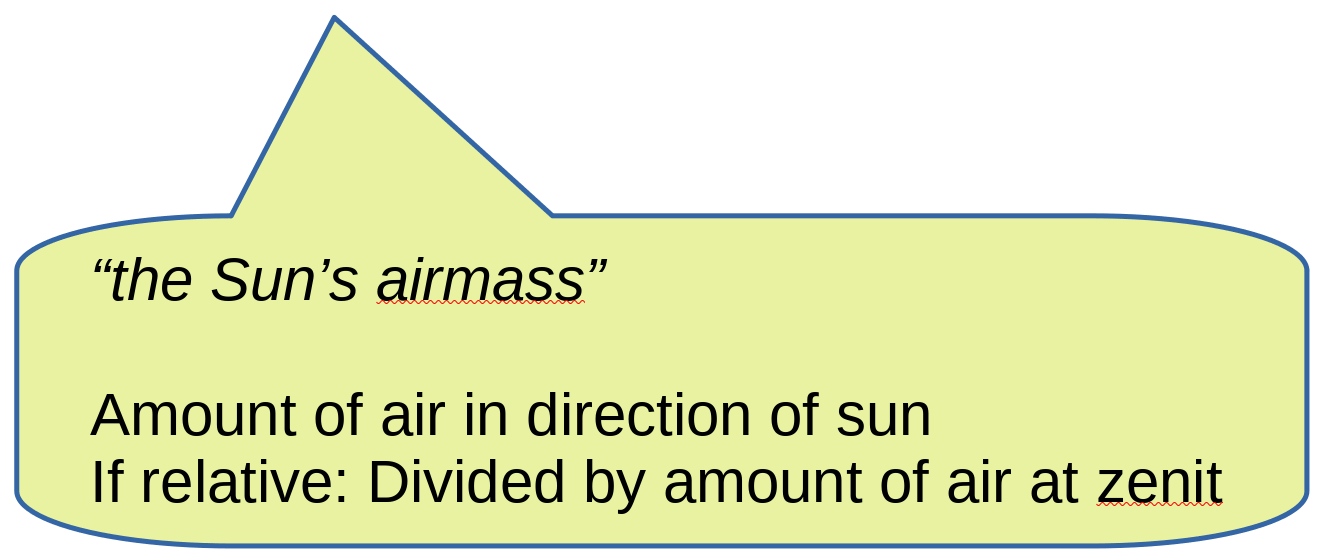
\includegraphics[width=0.5\textwidth]{bubble.png}};}
    \onslide<3>{\node at (1.5, -2.1) {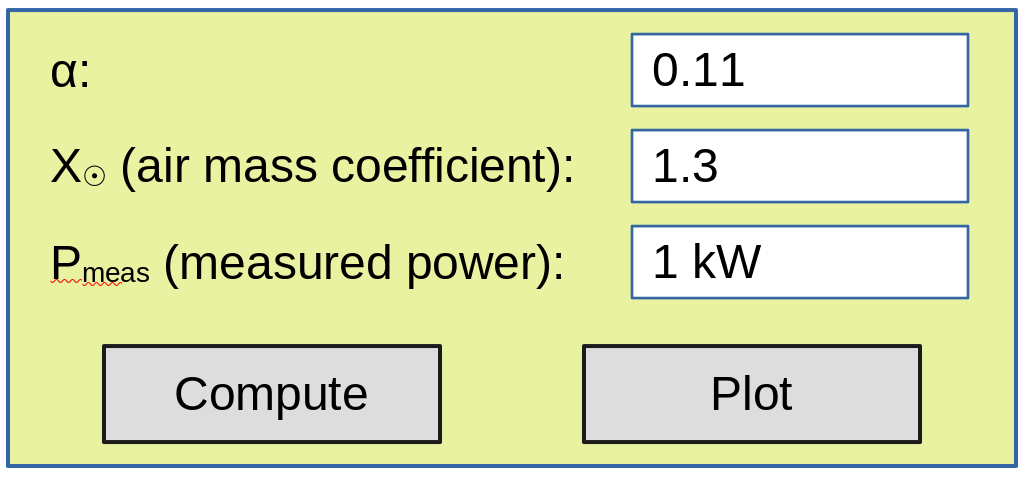
\includegraphics[width=0.5\textwidth]{compute.png}};}
    \end{tikzpicture}
%     \begin{itemize}
%         \item Computable formulae
%         \item Screen readers
%         \item Active documents
%         \item Formula search
%     \end{itemize}
\end{frame}


\begin{frame}
    \frametitle{Motivation: semantic services}
    \centering
    \Large
    For all those services\\
    {\bfseries we need semantic annotations!}\\\com{(full formalization not necessary)}
    \vspace{2em}\par
    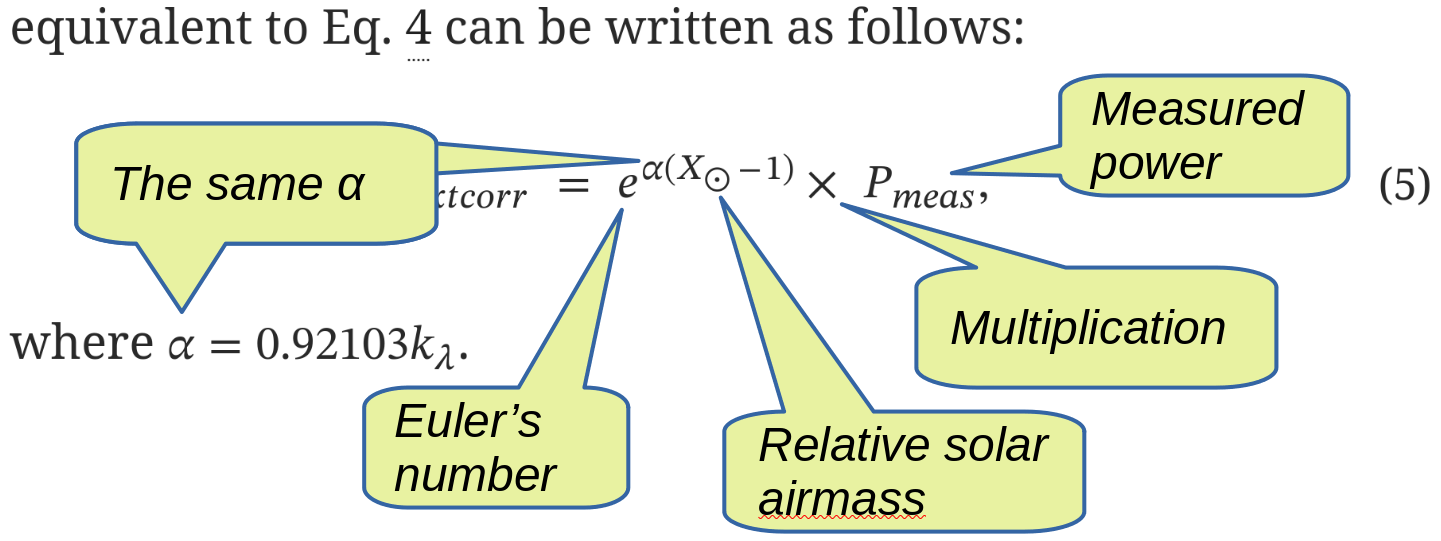
\includegraphics[width=0.5\textwidth]{annos.png}
    \vspace{2em}\par
    \pause
    Authors don't provide them $\leadsto$ We have to infer them
\end{frame}


